\chapterWithSubtitle{Universal Turing Machines}{February 18, 2021}

\section{Equivalent Turing Machine Variants}
\begin{itemize}
    \item Standard turing machine (single infinite tape)
    \item Multi-track tapes
    \begin{itemize}
        \item Each column of tape input can be combined into one larger inputs
        \item Multiple tapes can represent binary input
        \item $\delta: Q \times \Gamma_1 \times \Gamma_2 \times \Gamma_3 \rightarrow Q \times \Gamma_1 \times \Gamma_2 \times \Gamma_3 \times \{ -1, +1 \}$
    \end{itemize}
    \item Doubly-infinite tape
    \begin{itemize}
        \item Can be modelled as a TM with multiple tracks (positive indexes on one tape, negative indexes on the other).
        \item Can be modelled as a TM with interweaving positive and negative indexes.
    \end{itemize}
    \item Multiple heads
    \begin{itemize}
        \item $\delta: Q^3 \times \Gamma^3 \rightarrow Q^3 \times \Gamma^3 \times \{ -1, 0, 1\}^3$
        \item This could easily be represented as a standard transition function by redefining the states, input symbols, and directions.
    \end{itemize}
    \item Multiple heads and tapes
    \begin{itemize}
        \item $Q_1 \times Q_2 \times Q_3 \times \Gamma_1 \times \Gamma_2 \times \Gamma_3 \rightarrow Q_1 \times Q_2 \times Q_3 \times \Gamma_1 \times \Gamma_2 \times \Gamma_3 \times \{ -1, +1 \}^3$
    \end{itemize}
\end{itemize}

\section{Universal Turing Machine}

\subsection{Special Purpose Machines}
\begin{itemize}
    \item Different DFAs are needed for different languages.
    \item Similarly, different TMs are needed for different languages.
    \item Early computers were no different.
\end{itemize}

\subsection{Universal Turing Machine}
\begin{itemize}
    \item A single TM $M_u$ that can compute anything computable.
    \item Takes as input:
    \begin{itemize}
        \item the description of some other TM $M$
        \item data $w$ for $M$ to run on
    \end{itemize}
    \item Outputs:
    \begin{itemize}
        \item results of running $M(w)$
    \end{itemize}
\end{itemize}

\subsection{Coding of TMs}
\begin{itemize}
    \item Show how to represent every TM as a natural number
    \item \textit{Lemma}: If $L$ over alphabet $\{ 0, 1 \}$ is accepted by some TM $M$, then there is a one-tape TM that accepts $L$ such that:
    \begin{itemize}
        \item $\Gamma = \{ 0, 1, B \}$
        \item states numbered $1, ..., k$
        \item $q_1$ is a unique start state
        \item $q_2$ is a unique halt/accept state
        \item $q_3$ is a unique halt/reject state
    \end{itemize}
    \item So to represent a TM, we need only list its set of transitions - everything else is implicit by the above.
\end{itemize}

\subsection{Encoding Alphabet and States}
\begin{itemize}
    \item Each character in $\Gamma$ is mapped to a unique binary string.
    \item Each state in $Q$ is mapped to a unique binary string. Note that these binary strings can be the same as the $\Gamma$ binary strings.
    \item To encode $\delta(q_\text{old}, \$) = (q_\text{start}, \$, \text{right})$, we would write $100 \cdot 011 \mid 001 \cdot 011 \cdot 1$ or simply $100011 \mid 0010111$, using the corresponding binary string.
    \item All the transition strings are concatenated to define the transition function as a binary string.
\end{itemize}

\subsection{Encoding the Initial State}
\begin{itemize}
    \item The TM $M$ is encoded as a string. $M_u(M, w)$ needs to accept if $M(w)$ accepts, and reject if $M(w)$ rejects.
    \item Instead of directly encoding the input string, each character is padded to the right with a string of $0$s that will later be replaced by a state binary string.
    \item The first string of $0$s is changed to the start state.
    \item The string of $0$s represents a state that the head is not at. Only one character will not have a corresponding string of $0$s.
\end{itemize}

\section{\textit{The} Universal Turing Machine}

\subsection{$M_u$ Operation Concept}
\begin{itemize}
    \item We assume without a loss of generality that our universal turing machine $M_u$ has two tapes and two heads:
    \begin{itemize}
        \item \textbf{Input tape}: stores the encoding of $\langle M \rangle = \langle \text{state}, \text{tape input}, \text{head position} \rangle$
        \item \textbf{Machine tape}: Encoding tape which stores $M$'s transition function.
    \end{itemize}
    \item \textbf{General Idea}: For any given configuration of $M$, our $M_u$ will:
    \begin{itemize}
        \item Starting from the leftmost of the input tape, scan the tape for the first state which is not $\langle \text{reject} \rangle$/$0$s.
        \item Scan the machine tape for the transition function that matches the substring found in the input tape.
        \item Based on the transition, it will write the right half of the transition function into the current input tape cell.
        \item Based on the head direction of the transition function, it will move the current state left or right.
    \end{itemize}
\end{itemize}

\subsection{Implications}
\begin{itemize}
    \item Every TM is encoded by a unique element of $N$ (where $N$ is a natural number).
    \item \textit{Convention}: elements of $N$ that do not correspond to any TM encoding represent the "null TM" that accepts nothing.
    \item Thus, every TM is a number, and vice versa.
    \item Let $\langle M \rangle$ mean the number that encodes $M$. Conversely, let $M_n$ be the TM with encoding $n$.
    \item \textit{Big Idea}: Every TM can be represented by a number (strings of $0$s and $1$s) and there exists a universal TM $M_u$ that can simulate any other TM.
    \item[] 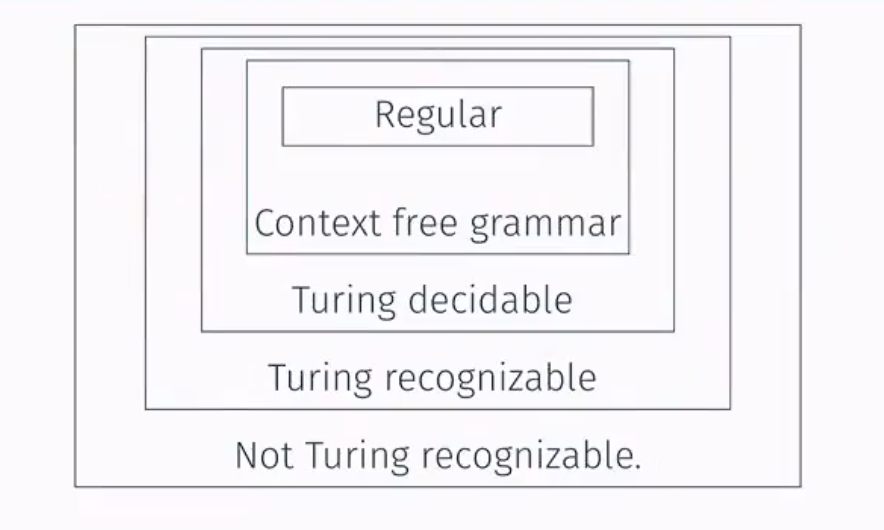
\includegraphics[width=\textwidth]{lecture9/images/turing-recognizable.png}
\end{itemize}
